% 三棱柱拓扑示意；投影不按比例。线型按源图：底面与可见侧棱、A'C'、A'C、AC' 实线，
% A'B'、B'C'、BB'、A'B、AC 虚线；B' 位于 A'C 下方。
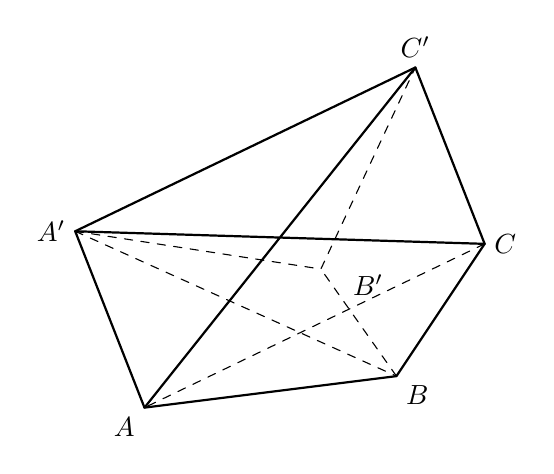
\begin{tikzpicture}[x=0.8cm,y=0.8cm,line cap=round,line join=round]
  \coordinate (A)  at (0,0);
  \coordinate (B)  at (4,0.5);
  \coordinate (C)  at (5.4,2.6);
  \coordinate (Ap) at (-1.1,2.8);
  \coordinate (Bp) at (2.8,2.2);
  \coordinate (Cp) at (4.3,5.4);
  % 底面三角形
  \draw[thick] (A)--(B)--(C);
  \draw[dashed] (C)--(A);
  % 上底面：A'C' 实线，其余两棱虚线
  \draw[thick] (Ap)--(Cp);
  \draw[dashed] (Ap)--(Bp)--(Cp);
  % 侧棱：AA'、CC' 实线，BB' 虚线
  \draw[thick] (A)--(Ap) (C)--(Cp);
  \draw[dashed] (B)--(Bp);
  % 两条对角实线 A'C、AC' 与虚线 A'B
  \draw[thick] (Ap)--(C) (A)--(Cp);
  \draw[dashed] (Ap)--(B);
  \node[below left] at (A) {$A$};
  \node[below right] at (B) {$B$};
  \node[right] at (C) {$C$};
  \node[left] at (Ap) {$A'$};
  \node at (3.55,1.95) {$B'$};
  \node[above] at (Cp) {$C'$};
\end{tikzpicture}
